
\chapter{针对存在未观测混杂因素的配对观察性研究的Rosenbaum式$p$值}
\chaptermark{配对研究中的敏感性分析}\label{sec::rosenbaum-sensitivity-analysis}


\citet{rosenbaum1987sensitivity}提出了一种适用于配对观察性研究的敏感性分析技术。虽然该方法也适用于一般的配对研究\citep{rosenbaum2002design}，但在一对一配对的情况下其理论最为完善。与\ref{chapter::evalue}章及\ref{chapter::sensitivity-ACE}章不同，Rosenbaum式敏感性分析最适用于检验“不存在个体治疗效果”这一明确零假设的配对观察性研究。  


\section{基于配对数据的敏感性分析模型}


考虑一项配对观察性研究，用$(i,j)$表示第$i$对中的第$j$个单位$(i=1,\ldots, n; j=1,2)$。精确匹配时，单位$(i, 1)$与单位$(i, 2)$具有相同的协变量$X_i$。假设抽样独立同分布，并推广定义\ref{def::pscore}，将倾向得分定义为
$$
e_{ij} = \pr\{  Z_{ij} = 1\mid X_i, Y_{ij}(1), Y_{ij}(0) \} .
$$
令$\mathbb{S}_i = \{Y_{i1}(1), Y_{i1}(0), Y_{i2}(1), Y_{i2}(0)\}$表示第$i$对中全部潜在结果的集合。在给定事件$Z_{i1} + Z_{i2} = 1$后，
\begin{eqnarray*}
\pi_{i1} &=& \pr\{ Z_{i1} = 1 \mid X_i, \mathbb{S}_i, Z_{i1} + Z_{i2} = 1 \} \\
&=& \frac{ \pr\{ Z_{i1} = 1, Z_{i2} = 0  \mid X_i, \mathbb{S}_i \} }
{ \pr\{ Z_{i1} + Z_{i2} = 1 \mid X_i, \mathbb{S}_i \} } \\
&=& \frac{ \pr\{ Z_{i1} = 1, Z_{i2} = 0  \mid X_i, \mathbb{S}_i \} }{ 
\pr\{ Z_{i1} = 1, Z_{i2} = 0 \mid X_i, \mathbb{S}_i \} + \pr\{ Z_{i1} = 0, Z_{i2} = 1 \mid X_i, \mathbb{S}_i \}
}\\
%{ \left[ \splitfrac{ \pr\{ Z_{i1} = 1, Z_{i2} = 0 \mid X_i, \mathbb{S}_i \} }
%{+\pr\{ Z_{i1} = 0, Z_{i2} = 1 \mid X_i, \mathbb{S}_i \} } \right] } \\
&=& \frac{  e_{i1} (1-e_{i2}) }{ e_{i1} (1-e_{i2}) + (1-e_{i1}) e_{i2}} 
\end{eqnarray*}
定义$o_{ij} = e_{ij} / (1 - e_{ij})$为单位$(i,j)$接受处理的优势，则
$$
\pi_{i1}  = \frac{o_{i1}}{  o_{i1} + o_{i2} } . 
$$
在可忽略性下，$e_{ij}$仅为$X_i$的函数，因此$e_{i1} = e_{i2}$且$\pi_{i1} = 1/2 $。于是，在给定协变量和潜在结果后，处理分配机制等价于处理与对照概率相等的配对实验。这就是第\ref{sec::ideal-matching-mpe}章讨论的分析配对观察性研究的一种策略。 


一般而言，$e_{ij}$还受未观测潜在结果影响，其值可在$0$到$1$之间变化。\citet{rosenbaum1987sensitivity}提出的敏感性分析模型对比值$o_{i1}/o_{i2} $设定了上下限。 

\begin{assumption}[Rosenbaum敏感性分析模型]\label{assume::rosenbaum-sensitivity}
优势比满足以下约束条件：
$$
o_{i1}/o_{i2} \leq \Gamma,\quad
o_{i2}/o_{i1} \leq \Gamma, \quad (i=1, \ldots, n)
$$
其中$\Gamma \geq  1$为预先给定的常数。等价地，
$$ 
\frac{1}{1+\Gamma } \leq 
\pi_{i1} \leq \frac{\Gamma}{1+\Gamma} \quad (i=1, \ldots, n)
$$
同样由$\Gamma \geq  1$决定。
\end{assumption}


在假设\ref{assume::rosenbaum-sensitivity}下，我们得到处理组与对照组概率不均等且随配对变化的偏倚MPE模型。当$\Gamma = 1$时，$\pi_{i1} = 1/2 $，即恢复为标准MPE模型。因此$\Gamma > 1$的数值大小反映了因匹配过程中遗漏变量而导致的对理想MPE模型的偏离程度。 
 
 
 
 \section{Rosenbaum敏感性分析模型下的最坏情况$p$值}


考虑基于对内差
$
\hat{\tau}_i = (2Z_{i1} - 1) (Y_{i1} - Y_{i2}) \  (i=1,\ldots, n). 
$
检验尖锐零假设
$$
\HF: Y_{ij}(1) = Y_{ij}(0) \text{ for } i = 1,\ldots, n \text{ and } j=1,2
$$
在$\HF$下，$|\hat{\tau}_i|$固定，但若$\hat{\tau}_i \neq 0$成立，$S_i = I(\hat{\tau}_i > 0)$仍是随机的。考虑以下一类检验统计量：
$$
T = \sumn S_i q_i,
$$
其中$q_i\geq 0$是$ (|\hat{\tau}_1|, \ldots, |\hat{\tau}_n|   ).$的函数。其特例包括符号统计量、配对$t$统计量（相差一个常数平移）以及 Wilcoxon 符号秩统计量：
$$
T = \sumn S_i,\quad T = \sumn S_i |\hat{\tau}_i|,\quad T = \sumn S_i R_i,
$$
其中$(R_1,\ldots, R_n)$是$ (|\hat{\tau}_1|, \ldots, |\hat{\tau}_n|   ).$的秩。 

对于一般的$\Gamma$，在假设\ref{assume::rosenbaum-sensitivity}下检验统计量$T$的零分布是什么？由于假设\ref{assume::rosenbaum-sensitivity}没有完全规定各$\pi_{i1}$的确切取值，答案可能很复杂。幸运的是，我们不需要知道$T$的确切分布，只需要知道在假设\ref{assume::rosenbaum-sensitivity}下使$p$值最大的$T$的最坏情形分布。该分布对应于
$$
S_i \iidsim  \text{Bernoulli}\left(  \frac{ \Gamma}{ 1+\Gamma} \right).
$$
此时$T$的均值为
$$
E_\Gamma( T ) = \frac{\Gamma}{1+\Gamma} \sumn q_i, 
$$
方差为
$$
\var_\Gamma( T ) = \frac{\Gamma}{(1+\Gamma)^2} \sumn q_i^2,
$$
并具有如下正态分布近似：
$$
\frac{T -\frac{\Gamma}{1+\Gamma} \sumn q_i }{ \sqrt{ \frac{\Gamma}{(1+\Gamma)^2} \sumn q_i^2  }} \rightarrow  \N01 
$$
这里的收敛为依分布收敛。在实践中，可以将一系列$p$值报告为$\Gamma$的函数。 


\section{实例演示}

\subsection{再探LaLonde数据集}\label{sec::rosenbaum-gamma-examples}

 

我们在配对后的LaLonde数据集上实施Rosenbaum式敏感性分析。利用\ri{Matching}包可构建配对数据集： 
\begin{lstlisting}
library("Matching")
library("sensitivitymv")
library("sensitivitymw")
dat <- read.table("cps1re74.csv",header=T)
dat$u74 <- as.numeric(dat$re74==0)
dat$u75 <- as.numeric(dat$re75==0)
y = dat$re78
z = dat$treat
x = as.matrix(dat[, c("age", "educ", "black",
                      "hispan", "married", "nodegree",
                      "re74", "re75", "u74", "u75")])
matchest = Match(Y = y, Tr = z, X = x)
ytreated = y[matchest$index.treated]
ycontrol = y[matchest$index.control]
datamatched = cbind(ytreated, ycontrol)
\end{lstlisting}

考虑使用检验统计量$T = \sumn S_i | \hat{\tau}_i |$。理想配对实验满足$\Gamma = 1$，此时可模拟$T$的分布，得到$p$值$0.002$，见图\ref{fg::lalonde_gamma}的第一个子图。将$\Gamma = 1.1$略微增大后，$T$的最坏情形分布向右移动，$p$值增至$0.011$。若进一步将$\Gamma$增至$1.3$，$T$的最坏情形分布将继续移动，$p$值超过$0.05$。图\ref{fg::p-gamma-lalonde}给出了各$\hat{\tau}_i$的直方图及$p$值随$\Gamma$变化的曲线；$\Gamma  = 1.233$衡量了在$0.05$水平上仍能拒绝零假设时所容许的最大混杂程度。 

也可用\ri{sensitivitymw}包中的\ri{senmw}函数，求出一系列随$\Gamma$变化的$p$值。
\begin{lstlisting}
Gamma  = seq(1, 1.4, 0.001)
Pvalue = Gamma
for(i in 1:length(Gamma))
{
  Pvalue[i] = senmw(datamatched, gamma = Gamma[i], 
                    method = "t")$pval
}
\end{lstlisting}
图\ref{fg::p-gamma-lalonde}给出了$p$值随$\Gamma$变化的曲线。 

 
 
 
 



\begin{figure}
\centering
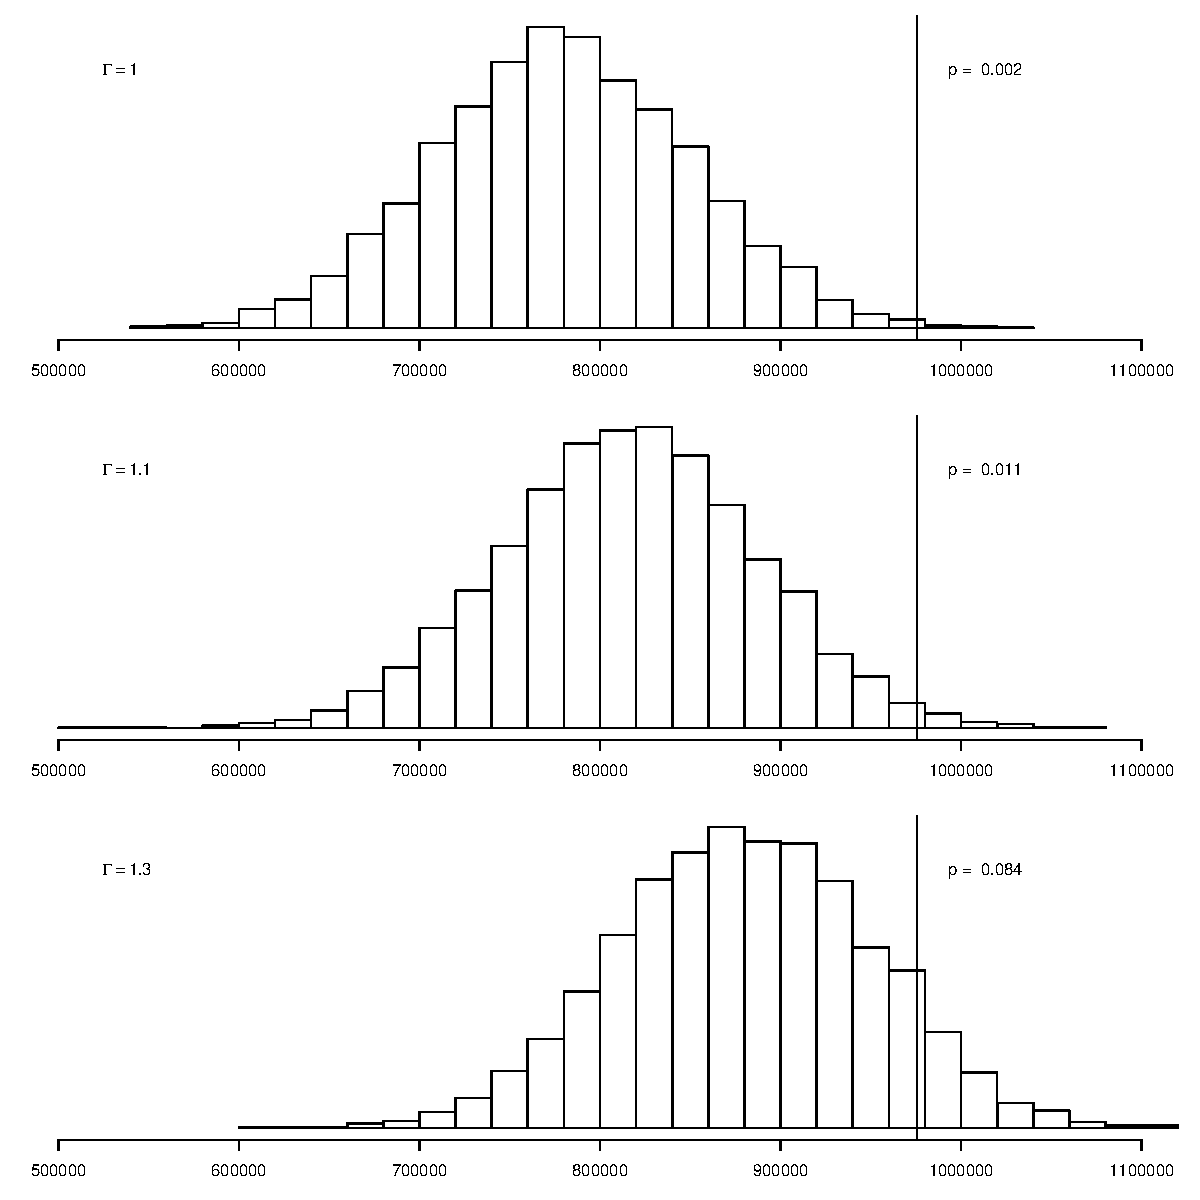
\includegraphics[width =  \textwidth]{figures/lalonde_hist_gamma.pdf}
\caption{基于配对LaLonde数据，满足$S_i$服从独立同分布Bernoulli$(\Gamma/(1+\Gamma))$时$T = \sumn S_i | \hat{\tau}_i |$的最坏情况分布。}\label{fg::lalonde_gamma}
\end{figure} 
 
 
 
 \begin{figure}
\centering
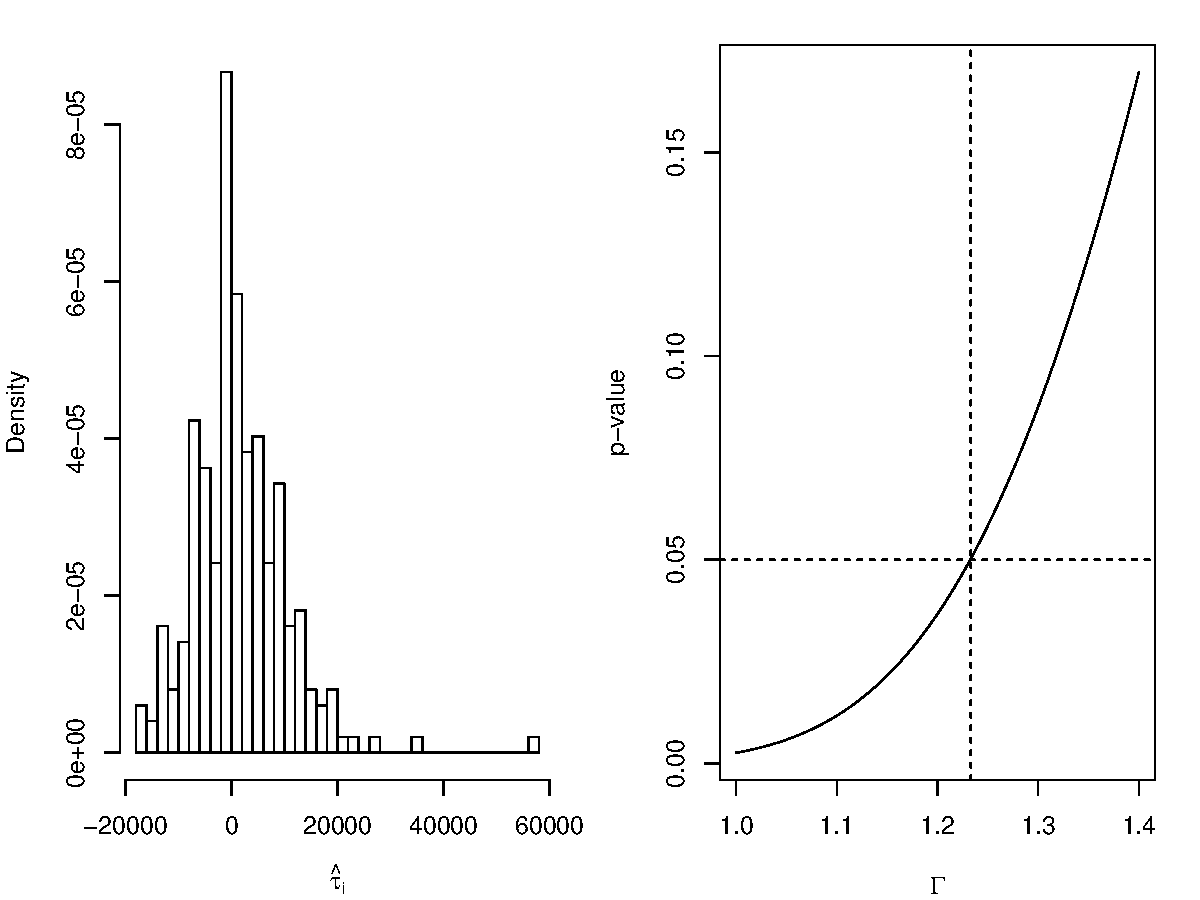
\includegraphics[width = \textwidth]{figures/lalonde_p_gamma.pdf}
\caption{基于配对LaLonde数据，$p$值随$\Gamma$的变化趋势。}\label{fg::p-gamma-lalonde}
\end{figure}



 
 
\subsection{Rosenbaum相关数据包中的两个实例} 

 

 \texttt{erpcp}数据集来自\ri{R}包\texttt{sensitivitymw}，其中包含根据观测协变量年龄与吸烟情况匹配的$n=39$对焊工和对照。结果为 DNA 洗脱率。图\ref{fg::another2sensitivity}(a) 给出了结果对内差的直方图，以及基于配对$t$统计量的$p$值随$\Gamma$变化的曲线。以下\ri{R}代码生成图\ref{fig::erpcp}。
 
 
\begin{lstlisting}
par(mfrow = c(1, 2), mai = c(0.8, 0.8, 0.3, 0.3))
data(erpcp)
hist(erpcp[, 1] - erpcp[, 2], main = "erpcp",
     xlab = expression(hat(tau)[i]),
     freq = FALSE)

Gamma  = seq(1, 5, 0.005)
Pvalue = Gamma
for(i in 1:length(Gamma))
{
  Pvalue[i] = senmw(erpcp, gamma = Gamma[i], method = "t")$pval
}
gammastar = Gamma[which(Pvalue >= 0.05)[1]]
gammastar

plot(Pvalue ~ Gamma, type = "l", 
     xlab = expression(Gamma), 
     ylab = "p-value")
abline(h = 0.05, lty = 2)
abline(v = gammastar, lty = 2)
\end{lstlisting}


 \texttt{lead250}数据集来自\ri{R}包\texttt{sensitivitymw}，其中包含 NHANES 中按性别、年龄、种族、教育程度和家庭收入匹配的$n=250$对每日吸烟者与不吸烟对照。结果是以$\mu g/l$为单位的血铅水平。图\ref{fg::another2sensitivity}(b) 给出了结果对内差的直方图，以及基于配对$t$统计量的$p$值随$\Gamma$变化的曲线。以下\ri{R}代码生成图\ref{fig::ead250}。
 
 \begin{lstlisting}
par(mfrow = c(1, 2), mai = c(0.8, 0.8, 0.3, 0.3))
data(lead250)
hist(lead250[, 1] - lead250[, 2],
     main = "lead250",
     xlab = expression(hat(tau)[i]),
     freq = FALSE)

Gamma  = seq(1, 2.5, 0.001)
Pvalue = Gamma
for(i in 1:length(Gamma))
{
  Pvalue[i] = senmw(lead250, gamma = Gamma[i], method = "t")$pval
}
gammastar = Gamma[which(Pvalue >= 0.05)[1]]
gammastar

plot(Pvalue ~ Gamma, type = "l", 
     xlab = expression(Gamma), ylab = "p-value")
abline(h = 0.05, lty = 2)
abline(v = gammastar, lty = 2)
\end{lstlisting}


\begin{figure}
\centering 
\begin{subfigure}[b]{\textwidth}
                \centering
                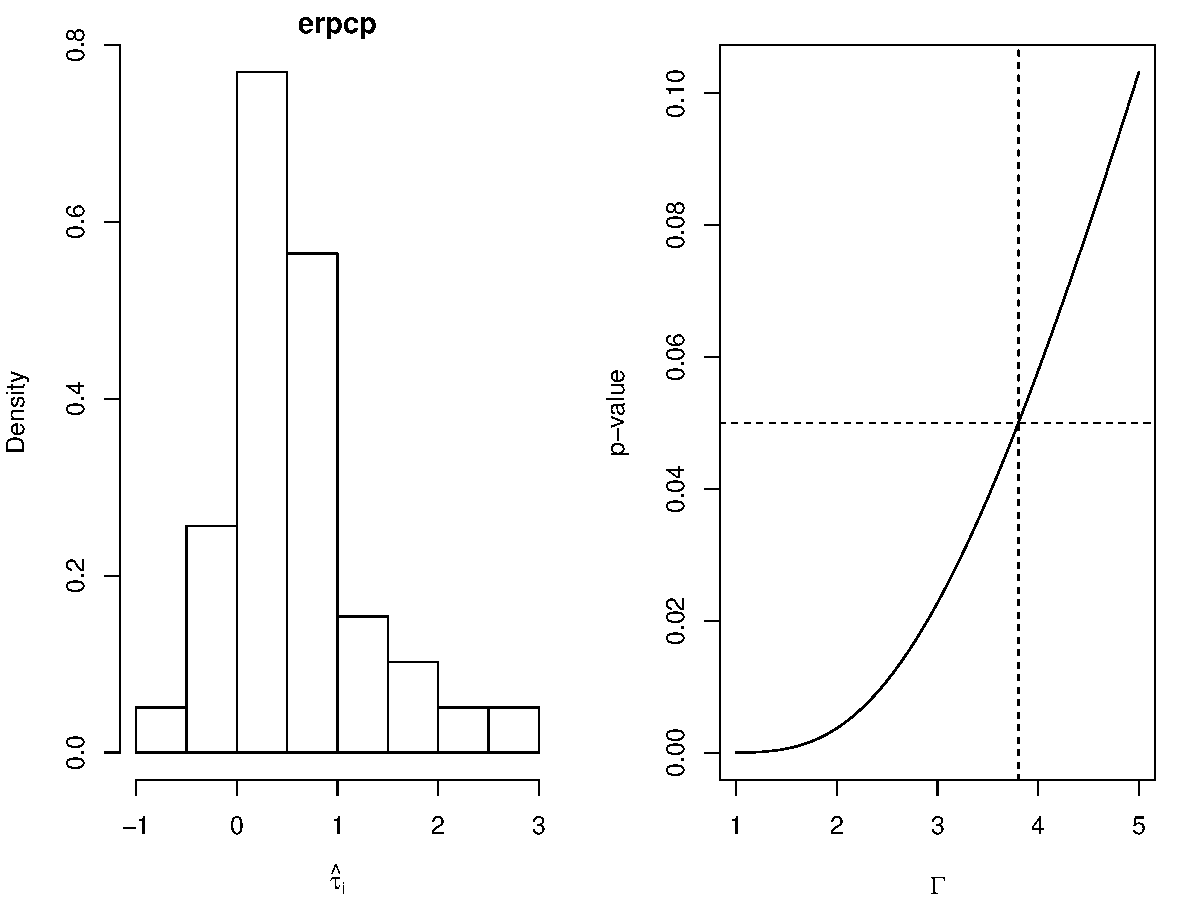
\includegraphics[width=\textwidth]{figures/erpcp_p_gamma.pdf}
                \caption{erpcp数据}
                \label{fig::erpcp}
        \end{subfigure}%
        
        
        
        
        
        
\begin{subfigure}[b]{\textwidth}
                \centering
                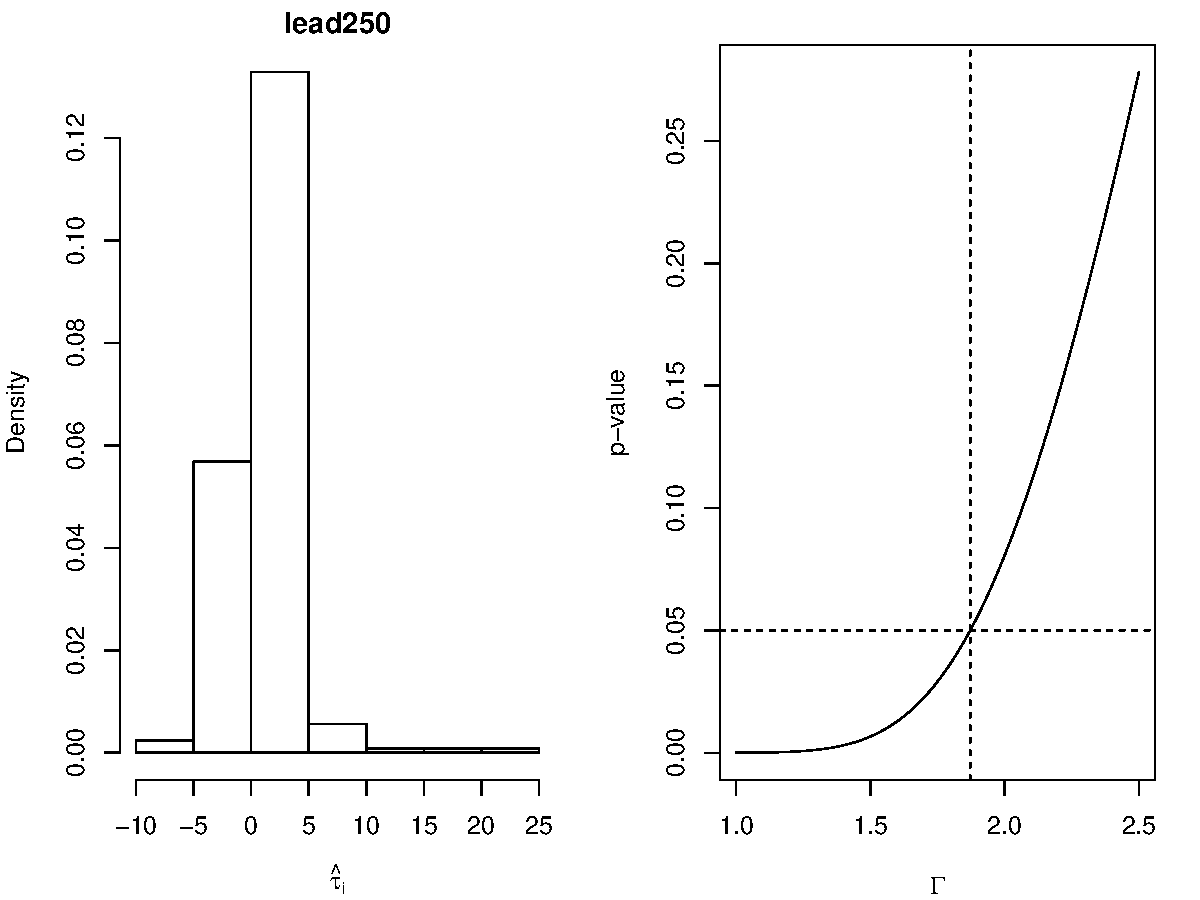
\includegraphics[width=\textwidth]{figures/lead250_p_gamma.pdf}
                \caption{ead250数据}
                \label{fig::ead250}
        \end{subfigure}%        
\caption{两个实例：$\hat{\tau}_i$分布直方图与$p$值随$\Gamma$的变化。}\label{fg::another2sensitivity}
\end{figure}


 
  

\section{作业习题}


\paragraph{假设\ref{assume::rosenbaum-sensitivity}的等价形式}\label{hw::rosenbaum-equivalent}

假设\ref{assume::rosenbaum-sensitivity}存在如下等价表述： 


\begin{assumption}
\label{assume::rosenbaum-equivalent}
倾向得分服从如下模型：
$$
\log \frac{  \pi_{ij} }{  1-\pi_{ij}  } = g(X_i) + \gamma U_{ij} ,\quad (i=1,\ldots, n; j=1,2)
$$
其中$g(\cdot)$为未知函数，$U_{ij} \in [0, 1]$为个体$(i, j)$的未观测协变量。 
\end{assumption}


证明：若假设\ref{assume::rosenbaum-equivalent}成立，则取$\Gamma = e^\gamma$时，假设\ref{assume::rosenbaum-sensitivity}必然成立。 


注：\citet[][page 108]{rosenbaum2002design}还证明，若假设\ref{assume::rosenbaum-sensitivity}成立，则存在一组$U_{ij}$使假设\ref{assume::rosenbaum-equivalent}成立。假设\ref{assume::rosenbaum-equivalent}可能更容易解释，因为$\gamma$衡量$U$对处理的条件对数优势比；逻辑回归系数的解释见第\ref{sec::logistic-regression}节。 



\paragraph{Rosenbaum方法的实践应用}
试运用基于配对的Rosenbaum法重新分析实例\ref{eg::chan-bmi-ATE}。



\paragraph{推荐阅读}


\citet{rosenbaum2015two}详细介绍了其开发的两个用于配对观察性研究敏感性分析的\ri{R}语言包使用教程。 

